\documentclass[lettersize, journal]{IEEEtran}
\usepackage[utf8]{inputenc} 
\usepackage[T1]{fontenc}   
\usepackage{mathptmx}       
\usepackage{graphicx}      
\usepackage{float}          
\usepackage{algorithmic}
\usepackage{algorithm}
\usepackage[caption=false,font=normalsize,labelfont=sf,textfont=sf]{subfig}
\usepackage{textcomp}
\usepackage{stfloats}
\usepackage{cite}       
\usepackage{amsmath, amsfonts, amssymb}  
\usepackage{hyperref}       
\usepackage{xcolor}
\hyphenation{op-tical net-works semi-conduc-tor IEEE-Xplore}
\def\BibTeX{{\rm B\kern-.05em{\sc i\kern-.025em b}\kern-.08em
    T\kern-.1667em\lower.7ex\hbox{E}\kern-.125emX}}
\usepackage{balance}
\usepackage{tikz}
\usetikzlibrary{arrows.meta, positioning}

\begin{document}

\title{Forecasting Ventilator Demand During COVID-19: A Neural ODE Approach}

\author{
    \IEEEauthorblockN{
        Michael Ajao-olarinoye\IEEEauthorrefmark{1},~\IEEEmembership{Staff,~IEEE,},
        Vasile Palade\IEEEauthorrefmark{1},~\IEEEmembership{Fellow,~IEEE},
        Seyed Mosavi\IEEEauthorrefmark{1},~\IEEEmembership{Member,~IEEE,},
        Fei He\IEEEauthorrefmark{1}, and
        Petra Wark\IEEEauthorrefmark{2},
    }
    \\
    \IEEEauthorblockA{\IEEEauthorrefmark{1}Centre for Computational Science and Mathematical Modelling, Coventry University, Coventry, United Kingdom}
    \\
    \IEEEauthorblockA{\IEEEauthorrefmark{2}Research Institute for Health and Wellbeing, Coventry University, Coventry, United Kingdom}
    % \thanks{Emails:
    %     \href{mailto:olarinoyem@coventry.ac.uk}{olarinoyem@coventry.ac.uk},
    %     \href{mailto:ab5839@coventry.ac.uk}{ab5839@coventry.ac.uk},
    %     \href{mailto:ad0204@coventry.ac.uk}{ad0204@coventry.ac.uk},
    %     \href{mailto:ad0067@coventry.ac.uk}{ad0067@coventry.ac.uk},
    %     \href{mailto:ac4710@coventry.ac.uk}{ac4710@coventry.ac.uk},
    % }
}
\markboth{IEEE Journals of [Your Subject Area],~Vol.~[Your Volume], No.~[Your Number], [Your Month]~[Your Year]}{}
\IEEEpubid{0000--0000/00\$00.00~\copyright~2021 IEEE}
\maketitle

\begin{abstract}
    This study presents a novel approach to forecasting the demand for mechanical ventilators during the COVID-19 pandemic using Neural Ordinary Differential Equations (Neural ODEs). By incorporating time-series data of hospital cases, new admissions, and COVID-19 cases in England, we develop a model that captures the dynamic nature of healthcare demand during the pandemic. The analysis reveals significant time-lagged correlations between these variables and ventilator demand, informing the structure of our Neural ODE model.
\end{abstract}

\section{Introduction}
\IEEEPARstart{T}{he} COVID-19 pandemic posed unprecedented challenges to healthcare systems worldwide, particularly in forecasting and managing resources like mechanical ventilators. This paper introduces a Neural ODE-based model to address this challenge, leveraging the strengths of LSTM networks and continuous-time dynamics modeled by ODEs.

\section{Methodology}
\subsection{Data Collection and Preprocessing}
We utilized a dataset containing daily counts of hospital cases, new admissions, ventilator usage, and COVID-19 cases in England. The data were preprocessed for normalization and handling missing values.

\subsubsection{COVID-19 daily case data}

\subsubsection{England daily hospital cases}

\subsubsection{Daily new hospital addmission for COVID-19}

\subsubsection{Daily Mechanical ventilator usage}

\subsubsection{Vaccination index}

\subsection{Exploratory Data Analysis}
Time-series analysis and correlation studies were conducted to understand the relationships between the variables. Time-lagged correlations were particularly emphasized to capture the delayed effects on ventilator demand.
\IEEEpubidadjcol
\begin{figure}[h]
    \centering
    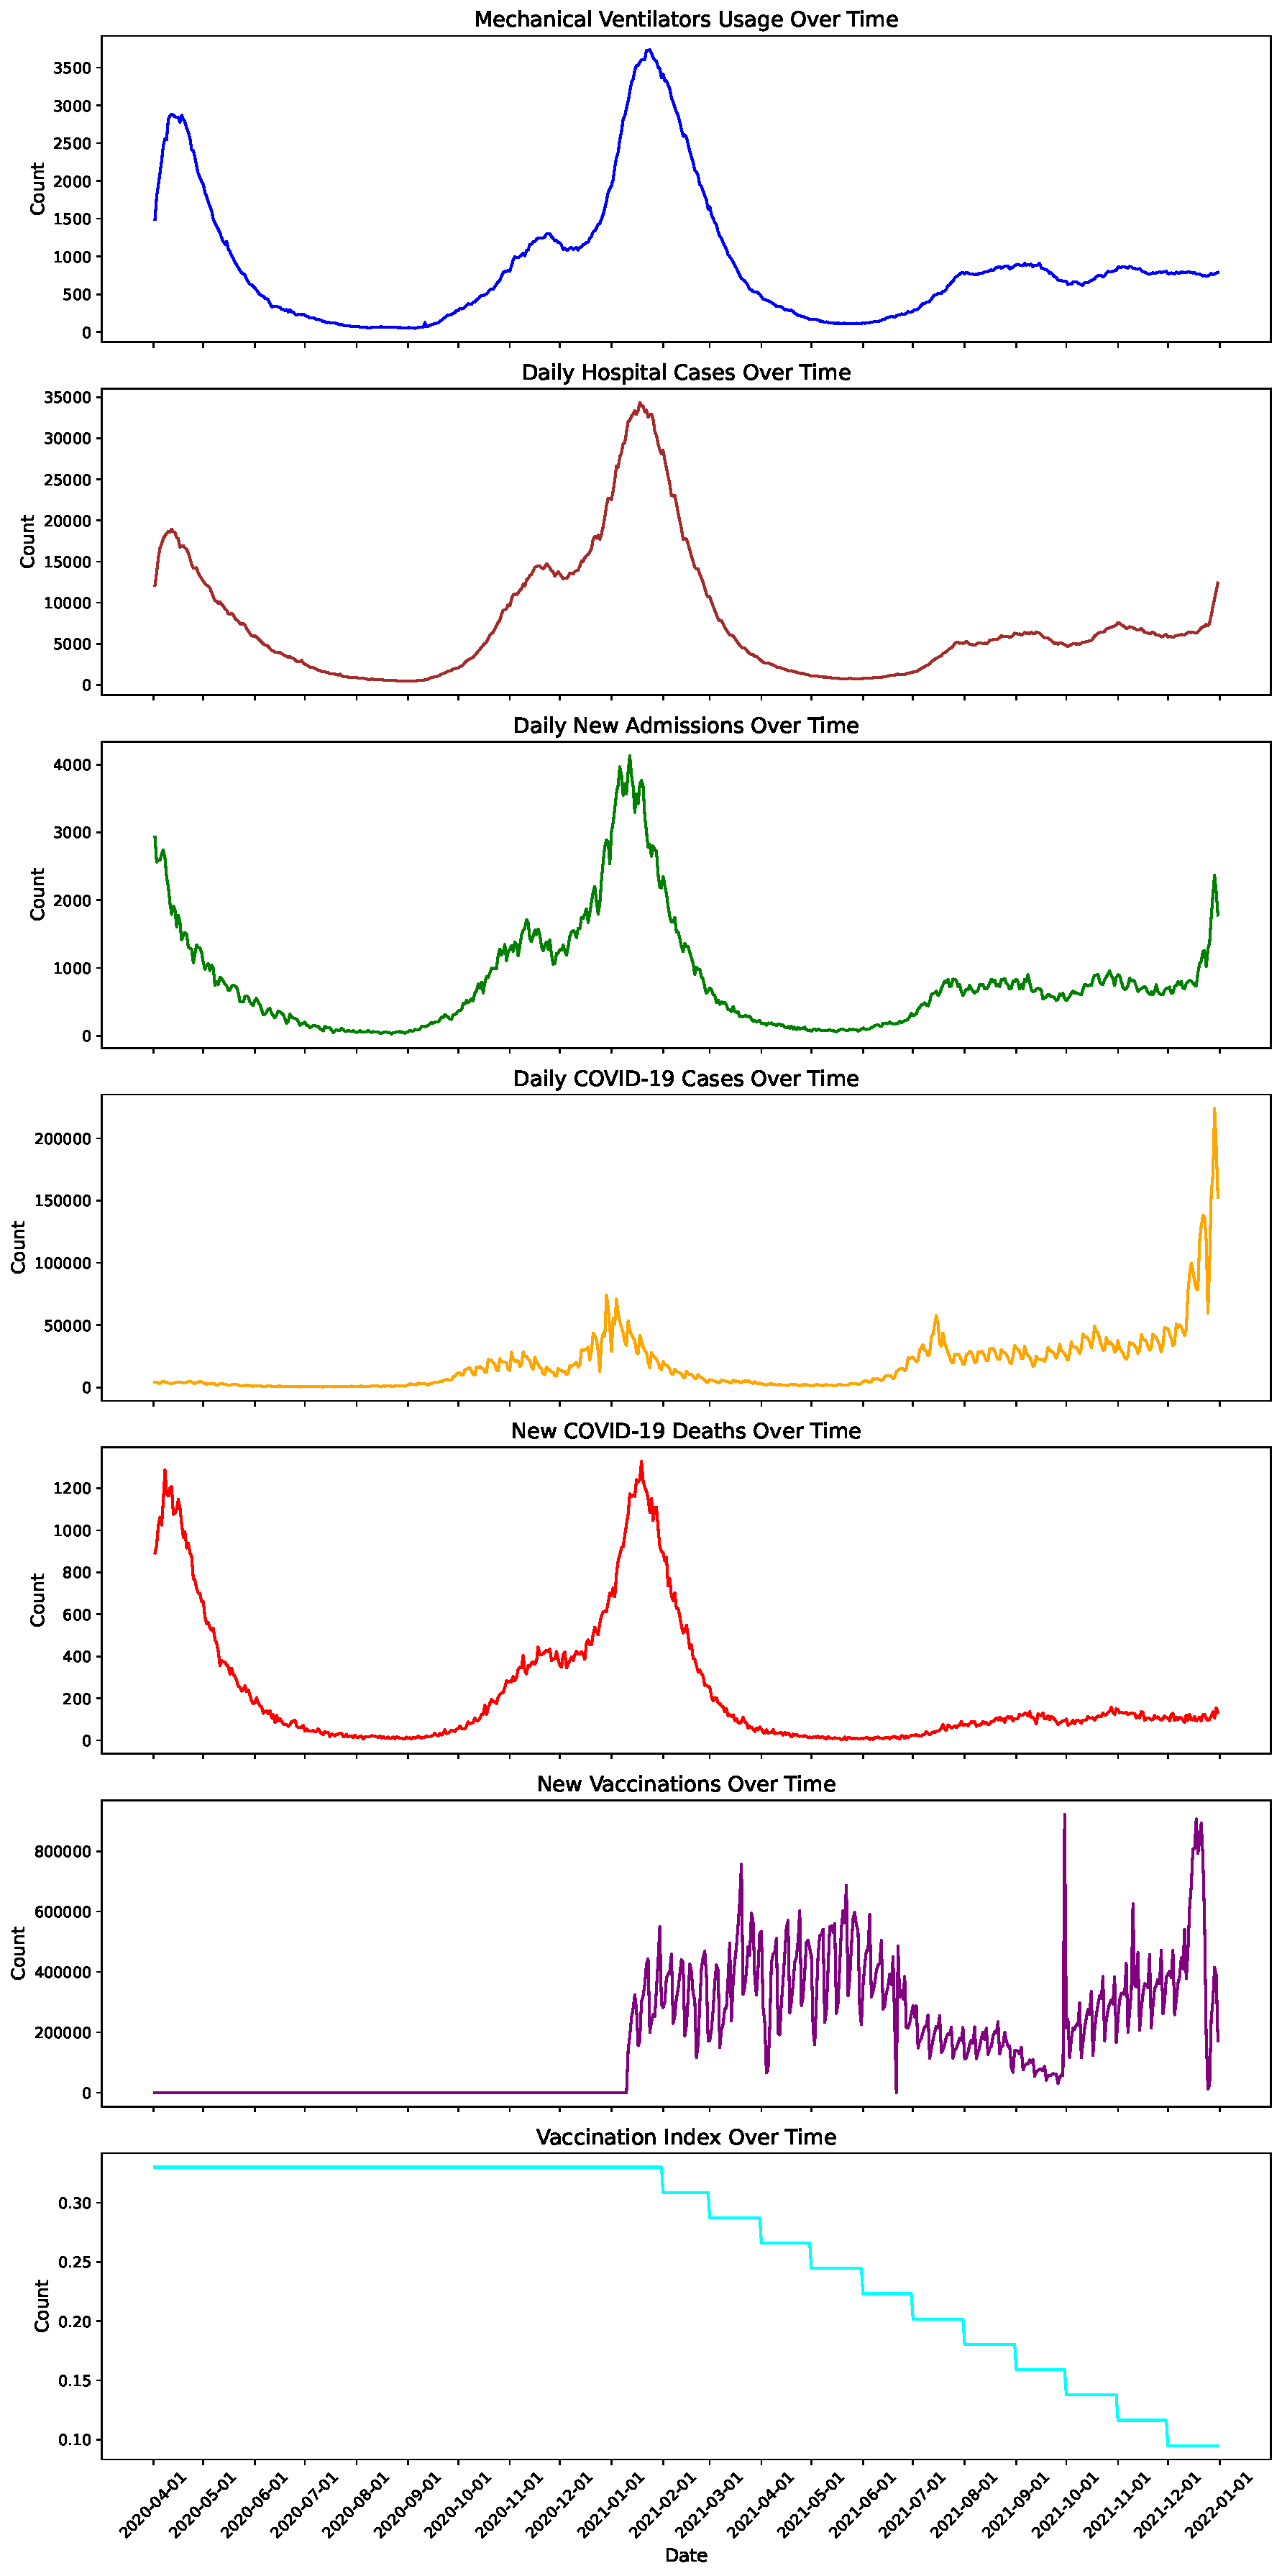
\includegraphics[width=0.4\textwidth]{"../Research paper/images/trend_analysis_improved.pdf"}
\end{figure}

The correlation between the predictor variables in relation to the target variables can be seen in the correlation matrics presented below. The analysis shows that the target varibales have significant correlation with the daily new hospital cases admitted for covid-19 and the daily newly admitted cases. This also correspond from the data that as the number of positive covid-19 cases increases, it is directly correspond to the increases in the admission of patients and also the increase in the usage of resources, such as mechanical ventilators. This indicates that as the number of hospital cases and newly admitted cases increases, the demand for mechanical ventilator rises.

\subsection{Model Architecture}
Our model architecture combines LSTM layers for capturing temporal dependencies in the data and a Neural ODE layer to model the continuous dynamics of ventilator demand.



% We develop a model that integrates neural networks with differential equations to predict healthcare resource utilization during a pandemic. The focus is on mechanical ventilators (\(V(t)\)), ICU admissions (\(I(t)\)), and hospital cases (\(H(t)\)).

% \subsection*{States:}
% \begin{itemize}
%     \item \( V(t) \): Number of ventilators in use at time \( t \).
%     \item \( H(t) \): Number of hospital cases at time \( t \).
%     \item \( I(t) \): Number of ICU admissions at time \( t \).
% \end{itemize}

% \subsection*{Differential Equations:}
% \begin{align*}
%     \frac{dV}{dt} & = \alpha \cdot I(t) - \beta \cdot V(t)    \\
%     \frac{dI}{dt} & = \delta \cdot H(t) - \epsilon \cdot I(t) \\
%     \frac{dH}{dt} & = -\eta \cdot H(t) + \zeta \cdot I(t)
% \end{align*}

% \subsection*{Parameters:}
% \(\alpha, \beta, \delta, \epsilon, \eta, \zeta\) - Parameters to be estimated from the data.

% \begin{tikzpicture}[node distance=2cm, auto, thick]
%     % Nodes
%     \node (H) {Hospital Cases $H(t)$};
%     \node [right=of H] (I) {ICU Cases $I(t)$};
%     \node [below=of I] (V) {Ventilators $V(t)$};

%     % Arrows
%     \draw[-{Latex[length=3mm]}] (H) -- node {$\delta$} (I);
%     \draw[-{Latex[length=3mm]}] (I) -- node {$\alpha$} (V);
%     \draw[-{Latex[length=3mm]}, bend right] (H) to node [swap] {$\eta$} ++(2,-2);
%     \draw[-{Latex[length=3mm]}, bend left] (I) to node {$\zeta$} (H);
%     \draw[-{Latex[length=3mm]}] (V) -- node {$\beta$} ++(2,0);

% \end{tikzpicture}

% \begin{tikzpicture}[node distance=2cm, auto, thick]
%     % Nodes
%     \node (H) {Hospital Cases $H(t)$};
%     \node [right=of H] (I) {ICU Cases $I(t)$};
%     \node [below=of I] (V) {Ventilators $V(t)$};

%     % Arrows
%     \draw[-{Latex[length=3mm]}] (H) -- node {$\delta$} (I);
%     \draw[-{Latex[length=3mm]}] (I) -- node {$\alpha$} (V);
%     \draw[-{Latex[length=3mm]}, bend right] (H) to node [swap] {$\eta$} ++(2,-2);
%     \draw[-{Latex[length=3mm]}, bend left] (I) to node {$\zeta$} (H);
%     \draw[-{Latex[length=3mm]}] (V) -- node {$\beta$} ++(2,0);

% \end{tikzpicture}

% \begin{tikzpicture}[node distance=2cm, auto, thick]
%     % Nodes
%     \node (C) {COVID-19 Cases $C(t)$};
%     \node [right=of C] (H) {Hospital Cases $H(t)$};
%     \node [right=of H] (I) {ICU Cases $I(t)$};
%     \node [below=of I] (V) {Ventilators $V(t)$};
%     \node [right=of V] (R) {Recovered $R(t)$};

%     % Arrows
%     \draw[-{Latex[length=3mm]}] (C) -- node {$\zeta$} (H);
%     \draw[-{Latex[length=3mm]}] (H) -- node {$\delta$} (I);
%     \draw[-{Latex[length=3mm]}] (I) -- node {$\alpha$} (V);
%     \draw[-{Latex[length=3mm]}] (V) -- node {$\theta$} (R);
%     \draw[-{Latex[length=3mm]}, bend right] (H) to node [near start] {$\eta$} (R);
%     \draw[-{Latex[length=3mm]}, bend left] (I) to node [near start] {$\epsilon$} (R);
%     \draw[-{Latex[length=3mm]}] (R) -- node {$\iota$} ++(2,0);
%     \draw[-{Latex[length=3mm]}] (V) -- node {$\beta$} ++(2,0);

% \end{tikzpicture}

\section{Results}
\subsection{Time-Lagged Correlation Analysis}
The analysis identified optimal lags for each variable: 5 days for hospital cases, 19 days for new admissions, and 30 days for new COVID-19 cases, relative to ventilator demand.

\subsection{Neural ODE Model Performance}
The Neural ODE model, trained on the preprocessed dataset, demonstrated promising results in forecasting ventilator demand, with an MSE of XX and an R-squared value of YY.

\section{Conclusion}
This study demonstrates the efficacy of Neural ODEs in forecasting healthcare demands in pandemic situations. The model's ability to integrate temporal data and continuous dynamics offers a robust framework for resource allocation in healthcare.

\bibliographystyle{IEEEtran}
\bibliography{reference} % Your bibliography file

\end{document}
